\chapter{Теоретические основы пространственной инвариантности в CNN} \label{theory}

\section{Формальное определение инвариантности к переносу}
\label{theory:formal_definition}

В данном разделе мы формализуем понятие инвариантности к переносу (или сдвигу) для функций и преобразований, а затем распространим эти определения на нейронные сети. Это позволит нам точно охарактеризовать проблему и разработать методы её количественной оценки.

\subsection{Инвариантность и эквивариантность функций}
\label{theory:formal_definition:invariance}

Начнем с общих определений инвариантности и эквивариантности для функций.

\begin{definition}[Инвариантность функции]
Пусть $f: X \rightarrow Y$ — функция, и $T: X \rightarrow X$ — преобразование, действующее на входном пространстве $X$. Функция $f$ называется инвариантной относительно преобразования $T$, если для любого $x \in X$ выполняется:
\begin{equation}
f(T(x)) = f(x)
\end{equation}
\end{definition}

Инвариантность означает, что результат функции не меняется при применении преобразования ко входу. Для задачи классификации изображений это означает, что вероятность принадлежности изображения определенному классу не должна меняться при сдвиге объекта.

\begin{definition}[Эквивариантность функции]
Пусть $f: X \rightarrow Y$ — функция, $T_X: X \rightarrow X$ — преобразование, действующее на входном пространстве $X$, и $T_Y: Y \rightarrow Y$ — преобразование, действующее на выходном пространстве $Y$. Функция $f$ называется эквивариантной относительно пары преобразований $(T_X, T_Y)$, если для любого $x \in X$ выполняется:
\begin{equation}
f(T_X(x)) = T_Y(f(x))
\end{equation}
\end{definition}

Эквивариантность означает, что преобразование входа приводит к предсказуемому преобразованию выхода. Для задачи детекции объектов это означает, что если объект смещается на изображении, то соответствующим образом должны смещаться и координаты предсказанной ограничивающей рамки.

Заметим, что инвариантность можно рассматривать как частный случай эквивариантности, когда $T_Y$ является тождественным преобразованием.

\subsection{Операторы сдвига для дискретных и непрерывных сигналов}
\label{theory:formal_definition:shift_operators}

Теперь конкретизируем эти определения для случая пространственных сдвигов в контексте обработки изображений.

Для непрерывных 2D-сигналов (изображений) $x \in L^2(\mathbb{R}^2)$ оператор сдвига $T_{\boldsymbol{\tau}}$ на вектор $\boldsymbol{\tau} = (\tau_x, \tau_y) \in \mathbb{R}^2$ определяется как:
\begin{equation}
[T_{\boldsymbol{\tau}}x](\mathbf{p}) = x(\mathbf{p} - \boldsymbol{\tau})
\end{equation}
где $\mathbf{p} = (p_x, p_y) \in \mathbb{R}^2$ — пространственные координаты.

Для дискретных изображений $x \in \mathbb{R}^{H \times W \times C}$, где $H$, $W$ — высота и ширина, а $C$ — число каналов, оператор целочисленного сдвига $T_{\boldsymbol{\delta}}$ на вектор $\boldsymbol{\delta} = (\delta_x, \delta_y) \in \mathbb{Z}^2$ определяется как:
\begin{equation}
[T_{\boldsymbol{\delta}}x]_{h,w,c} = x_{h-\delta_y, w-\delta_x, c}
\end{equation}
для всех допустимых индексов $h, w, c$, с соответствующими граничными условиями.

Однако в реальных задачах часто требуется выполнять субпиксельные (нецелочисленные) сдвиги. Для дискретных изображений это достигается путем интерполяции. Наиболее распространенные методы интерполяции включают:

\begin{itemize}
    \item Интерполяция ближайшего соседа:
    \begin{equation}
    [T_{\boldsymbol{\tau}}x]_{h,w,c} = x_{\lfloor h-\tau_y \rfloor, \lfloor w-\tau_x \rfloor, c}
    \end{equation}
    
    \item Билинейная интерполяция:
    \begin{align}
    [T_{\boldsymbol{\tau}}x]_{h,w,c} &= (1-\alpha)(1-\beta)x_{\lfloor h-\tau_y \rfloor, \lfloor w-\tau_x \rfloor, c} + \alpha(1-\beta)x_{\lfloor h-\tau_y \rfloor, \lfloor w-\tau_x \rfloor+1, c} \nonumber \\
    &+ (1-\alpha)\beta x_{\lfloor h-\tau_y \rfloor+1, \lfloor w-\tau_x \rfloor, c} + \alpha\beta x_{\lfloor h-\tau_y \rfloor+1, \lfloor w-\tau_x \rfloor+1, c}
    \end{align}
    где $\alpha = (w-\tau_x) - \lfloor w-\tau_x \rfloor$ и $\beta = (h-\tau_y) - \lfloor h-\tau_y \rfloor$ — дробные части координат.
\end{itemize}

\subsection{Инвариантность к переносу в контексте CNN}
\label{theory:formal_definition:cnn_context}

Рассмотрим сверточную нейронную сеть как функцию $f: \mathbb{R}^{H \times W \times C_{\text{in}}} \rightarrow \mathbb{R}^{D}$, которая отображает входное изображение $x$ в некоторое представление $f(x)$ (например, вектор вероятностей классов или карту признаков).

\begin{definition}[Строгая инвариантность CNN к сдвигу]
CNN $f$ называется строго инвариантной к сдвигу, если для любого входного изображения $x \in \mathbb{R}^{H \times W \times C_{\text{in}}}$ и любого сдвига $\boldsymbol{\tau} \in \mathbb{R}^2$ (с соответствующей обработкой краев) выполняется:
\begin{equation}
f(T_{\boldsymbol{\tau}}x) = f(x)
\end{equation}
\end{definition}

\begin{definition}[Строгая эквивариантность CNN к сдвигу]
CNN $f$, отображающая входное изображение в пространственное представление $f: \mathbb{R}^{H \times W \times C_{\text{in}}} \rightarrow \mathbb{R}^{H' \times W' \times C_{\text{out}}}$, называется строго эквивариантной к сдвигу, если для любого входного изображения $x$ и любого сдвига $\boldsymbol{\tau}$ существует соответствующий сдвиг $\boldsymbol{\tau}'$ такой, что:
\begin{equation}
f(T_{\boldsymbol{\tau}}x) = T_{\boldsymbol{\tau}'}f(x)
\end{equation}
где $\boldsymbol{\tau}' = \boldsymbol{\tau} / s$ для некоторого фактора масштабирования $s$, определяемого степенью даунсэмплинга в сети.
\end{definition}

Однако в реальных CNN строгая инвариантность или эквивариантность к произвольным сдвигам обычно не достигается из-за дискретной природы свертки и операций даунсэмплинга. Поэтому вводятся более практичные определения:

\begin{definition}[$\varepsilon$-приближенная инвариантность к сдвигу]
CNN $f$ называется $\varepsilon$-приближенно инвариантной к сдвигу, если для любого входного изображения $x$ и любого сдвига $\boldsymbol{\tau}$ из некоторого множества допустимых сдвигов $\mathcal{T}$ выполняется:
\begin{equation}
d(f(T_{\boldsymbol{\tau}}x), f(x)) \leq \varepsilon
\end{equation}
где $d$ — некоторая метрика в выходном пространстве (например, евклидово расстояние или косинусное расстояние), а $\varepsilon > 0$ — заданный порог.
\end{definition}

\begin{definition}[$\varepsilon$-приближенная эквивариантность к сдвигу]
CNN $f$, отображающая входное изображение в пространственное представление, называется $\varepsilon$-приближенно эквивариантной к сдвигу, если для любого входного изображения $x$ и любого сдвига $\boldsymbol{\tau} \in \mathcal{T}$ выполняется:
\begin{equation}
d(f(T_{\boldsymbol{\tau}}x), T_{\boldsymbol{\tau}'}f(x)) \leq \varepsilon
\end{equation}
где $\boldsymbol{\tau}' = \boldsymbol{\tau} / s$.
\end{definition}

Эти определения позволяют количественно измерять степень инвариантности или эквивариантности CNN к сдвигам. В частности, можно определить функцию несоответствия сдвига (translation discrepancy function, TDF) для CNN $f$ как:

\begin{equation}
\text{TDF}_f(x, \boldsymbol{\tau}) = d(f(T_{\boldsymbol{\tau}}x), f(x))
\end{equation}

для случая инвариантности, или:

\begin{equation}
\text{TDF}_f(x, \boldsymbol{\tau}) = d(f(T_{\boldsymbol{\tau}}x), T_{\boldsymbol{\tau}'}f(x))
\end{equation}

для случая эквивариантности.

\subsection{Квантификация инвариантности к сдвигу}
\label{theory:formal_definition:quantification}

Для практической оценки степени инвариантности CNN к сдвигам можно использовать различные метрики.

Для классификационных задач одной из наиболее информативных метрик является косинусное сходство между векторами признаков, полученными из оригинального и сдвинутого изображений:

\begin{equation}
\rho(x, T_{\boldsymbol{\tau}}x) = \frac{f(x) \cdot f(T_{\boldsymbol{\tau}}x)}{\|f(x)\| \cdot \|f(T_{\boldsymbol{\tau}}x)\|}
\end{equation}

где $f(x)$ и $f(T_{\boldsymbol{\tau}}x)$ — векторы признаков, извлеченные моделью из оригинального и сдвинутого изображений соответственно.

Альтернативной метрикой является изменение в распределении вероятностей классов:

\begin{equation}
\text{KL}(p_x \| p_{T_{\boldsymbol{\tau}}x}) = \sum_{k=1}^K p_x(k) \log \frac{p_x(k)}{p_{T_{\boldsymbol{\tau}}x}(k)}
\end{equation}

где $p_x$ и $p_{T_{\boldsymbol{\tau}}x}$ — распределения вероятностей классов для оригинального и сдвинутого изображений.

Для задач детекции объектов можно использовать следующие метрики:

\begin{itemize}
    \item Стабильность IoU:
    \begin{equation}
    \text{IoU-stability}(x, T_{\boldsymbol{\tau}}x) = \text{IoU}(B, T_{-\boldsymbol{\tau}}B')
    \end{equation}
    где $B$ — предсказанная ограничивающая рамка для оригинального изображения, $B'$ — предсказанная рамка для сдвинутого изображения, а $T_{-\boldsymbol{\tau}}$ — обратный сдвиг на вектор $-\boldsymbol{\tau}$.
    
    \item Дрейф центра:
    \begin{equation}
    \text{center-drift}(x, T_{\boldsymbol{\tau}}x) = \|\text{center}(B) - \text{center}(T_{-\boldsymbol{\tau}}B')\|_2
    \end{equation}
    
    \item Стабильность уверенности:
    \begin{equation}
    \text{confidence-stability}(x, T_{\boldsymbol{\tau}}x) = |c - c'|
    \end{equation}
    где $c$ и $c'$ — значения уверенности модели для предсказаний на оригинальном и сдвинутом изображениях.
\end{itemize}

В рамках данной работы мы будем использовать эти метрики для количественной оценки степени инвариантности различных архитектур CNN к субпиксельным сдвигам входных изображений.

\subsection{Теоретические границы инвариантности в дискретных CNN}
\label{theory:formal_definition:theoretical_bounds}

Важно отметить, что для дискретных CNN существуют теоретические ограничения на достижимую степень инвариантности к произвольным сдвигам. Эти ограничения связаны с дискретной природой сверточных операций и даунсэмплинга.

Как показано в работе Chaman и Dokmanic \cite{Chaman2021}, для CNN с фиксированными дискретными фильтрами и операциями даунсэмплинга существует нижняя граница функции несоответствия сдвига, которая зависит от величины субпиксельного сдвига и структуры сети.

В частности, для CNN $f$ с $L$ слоями, каждый из которых включает свертку и даунсэмплинг с фактором $s_l$, минимальное значение TDF для субпиксельного сдвига $\boldsymbol{\tau}$ удовлетворяет:

\begin{equation}
\min_{f \in \mathcal{F}} \max_{x \in \mathcal{X}, \boldsymbol{\tau} \in [0,1)^2} \text{TDF}_f(x, \boldsymbol{\tau}) \geq C \cdot \min_{l=1}^L \|\boldsymbol{\tau} \cdot \prod_{i=1}^{l-1} s_i \mod 1\|
\end{equation}

где $\mathcal{F}$ — класс всех CNN с заданной архитектурой, $\mathcal{X}$ — пространство входных изображений, а $C$ — константа, зависящая от структуры сети.

Это неравенство показывает, что для достижения инвариантности к произвольным субпиксельным сдвигам необходимо либо модифицировать архитектуру сети (например, используя методы анти-алиасинга), либо применять специальные методы обучения, которые минимизируют TDF для наиболее важных типов входных данных.

В следующих разделах мы рассмотрим, как различные архитектурные модификации, такие как BlurPool и TIPS, позволяют приблизиться к теоретическому пределу инвариантности к сдвигам для CNN.

\section{Вывод рецептивных полей в CNN}
\label{theory:receptive_fields}

\subsection{Определение и значимость рецептивных полей}
\label{theory:receptive_fields:definition}

Рецептивное поле (РП, Receptive Field) нейрона в сверточной нейронной сети — это область входного изображения, которая может повлиять на активацию данного нейрона. Размер рецептивного поля является ключевой характеристикой архитектуры CNN и имеет непосредственное отношение к её способности распознавать пространственные паттерны и демонстрировать инвариантность к смещениям.

\begin{definition}[Рецептивное поле]
Рецептивное поле $\mathcal{R}(l,i,j)$ нейрона с координатами $(i,j)$ в слое $l$ определяется как множество пикселей во входном изображении, изменение значений которых может повлиять на выход данного нейрона.
\end{definition}

Размер рецептивного поля обычно характеризуется его высотой и шириной в пикселях. Для современных глубоких CNN типичны большие рецептивные поля, охватывающие значительную часть входного изображения, что позволяет сети анализировать как локальные, так и глобальные признаки.

\subsection{Расчёт размера рецептивного поля}
\label{theory:receptive_fields:calculation}

Размер рецептивного поля нейрона зависит от нескольких архитектурных параметров: размеров ядер свертки, величины шага (stride) и дилатации в каждом слое CNN. Рассмотрим рекуррентную формулу для вычисления размера рецептивного поля.

Пусть для слоя $l$:
\begin{itemize}
    \item $k_l$ — размер ядра свертки
    \item $s_l$ — шаг свертки (stride)
    \item $d_l$ — коэффициент дилатации
\end{itemize}

Тогда эффективный размер ядра с учетом дилатации составляет:
\begin{equation}
k_l^{\text{eff}} = k_l + (k_l - 1)(d_l - 1)
\end{equation}

Определим размер рецептивного поля на слое $l$ как $r_l$. Для входного слоя $r_0 = 1$ (один пиксель). Для последующих слоев размер рецептивного поля можно рассчитать рекурсивно:

\begin{equation}
r_l = r_{l-1} + (k_l^{\text{eff}} - 1) \cdot \prod_{i=0}^{l-1} s_i
\end{equation}

Этот рекурсивный расчет позволяет определить размер рецептивного поля на любом уровне сети.

\begin{figure}[ht]
\centering
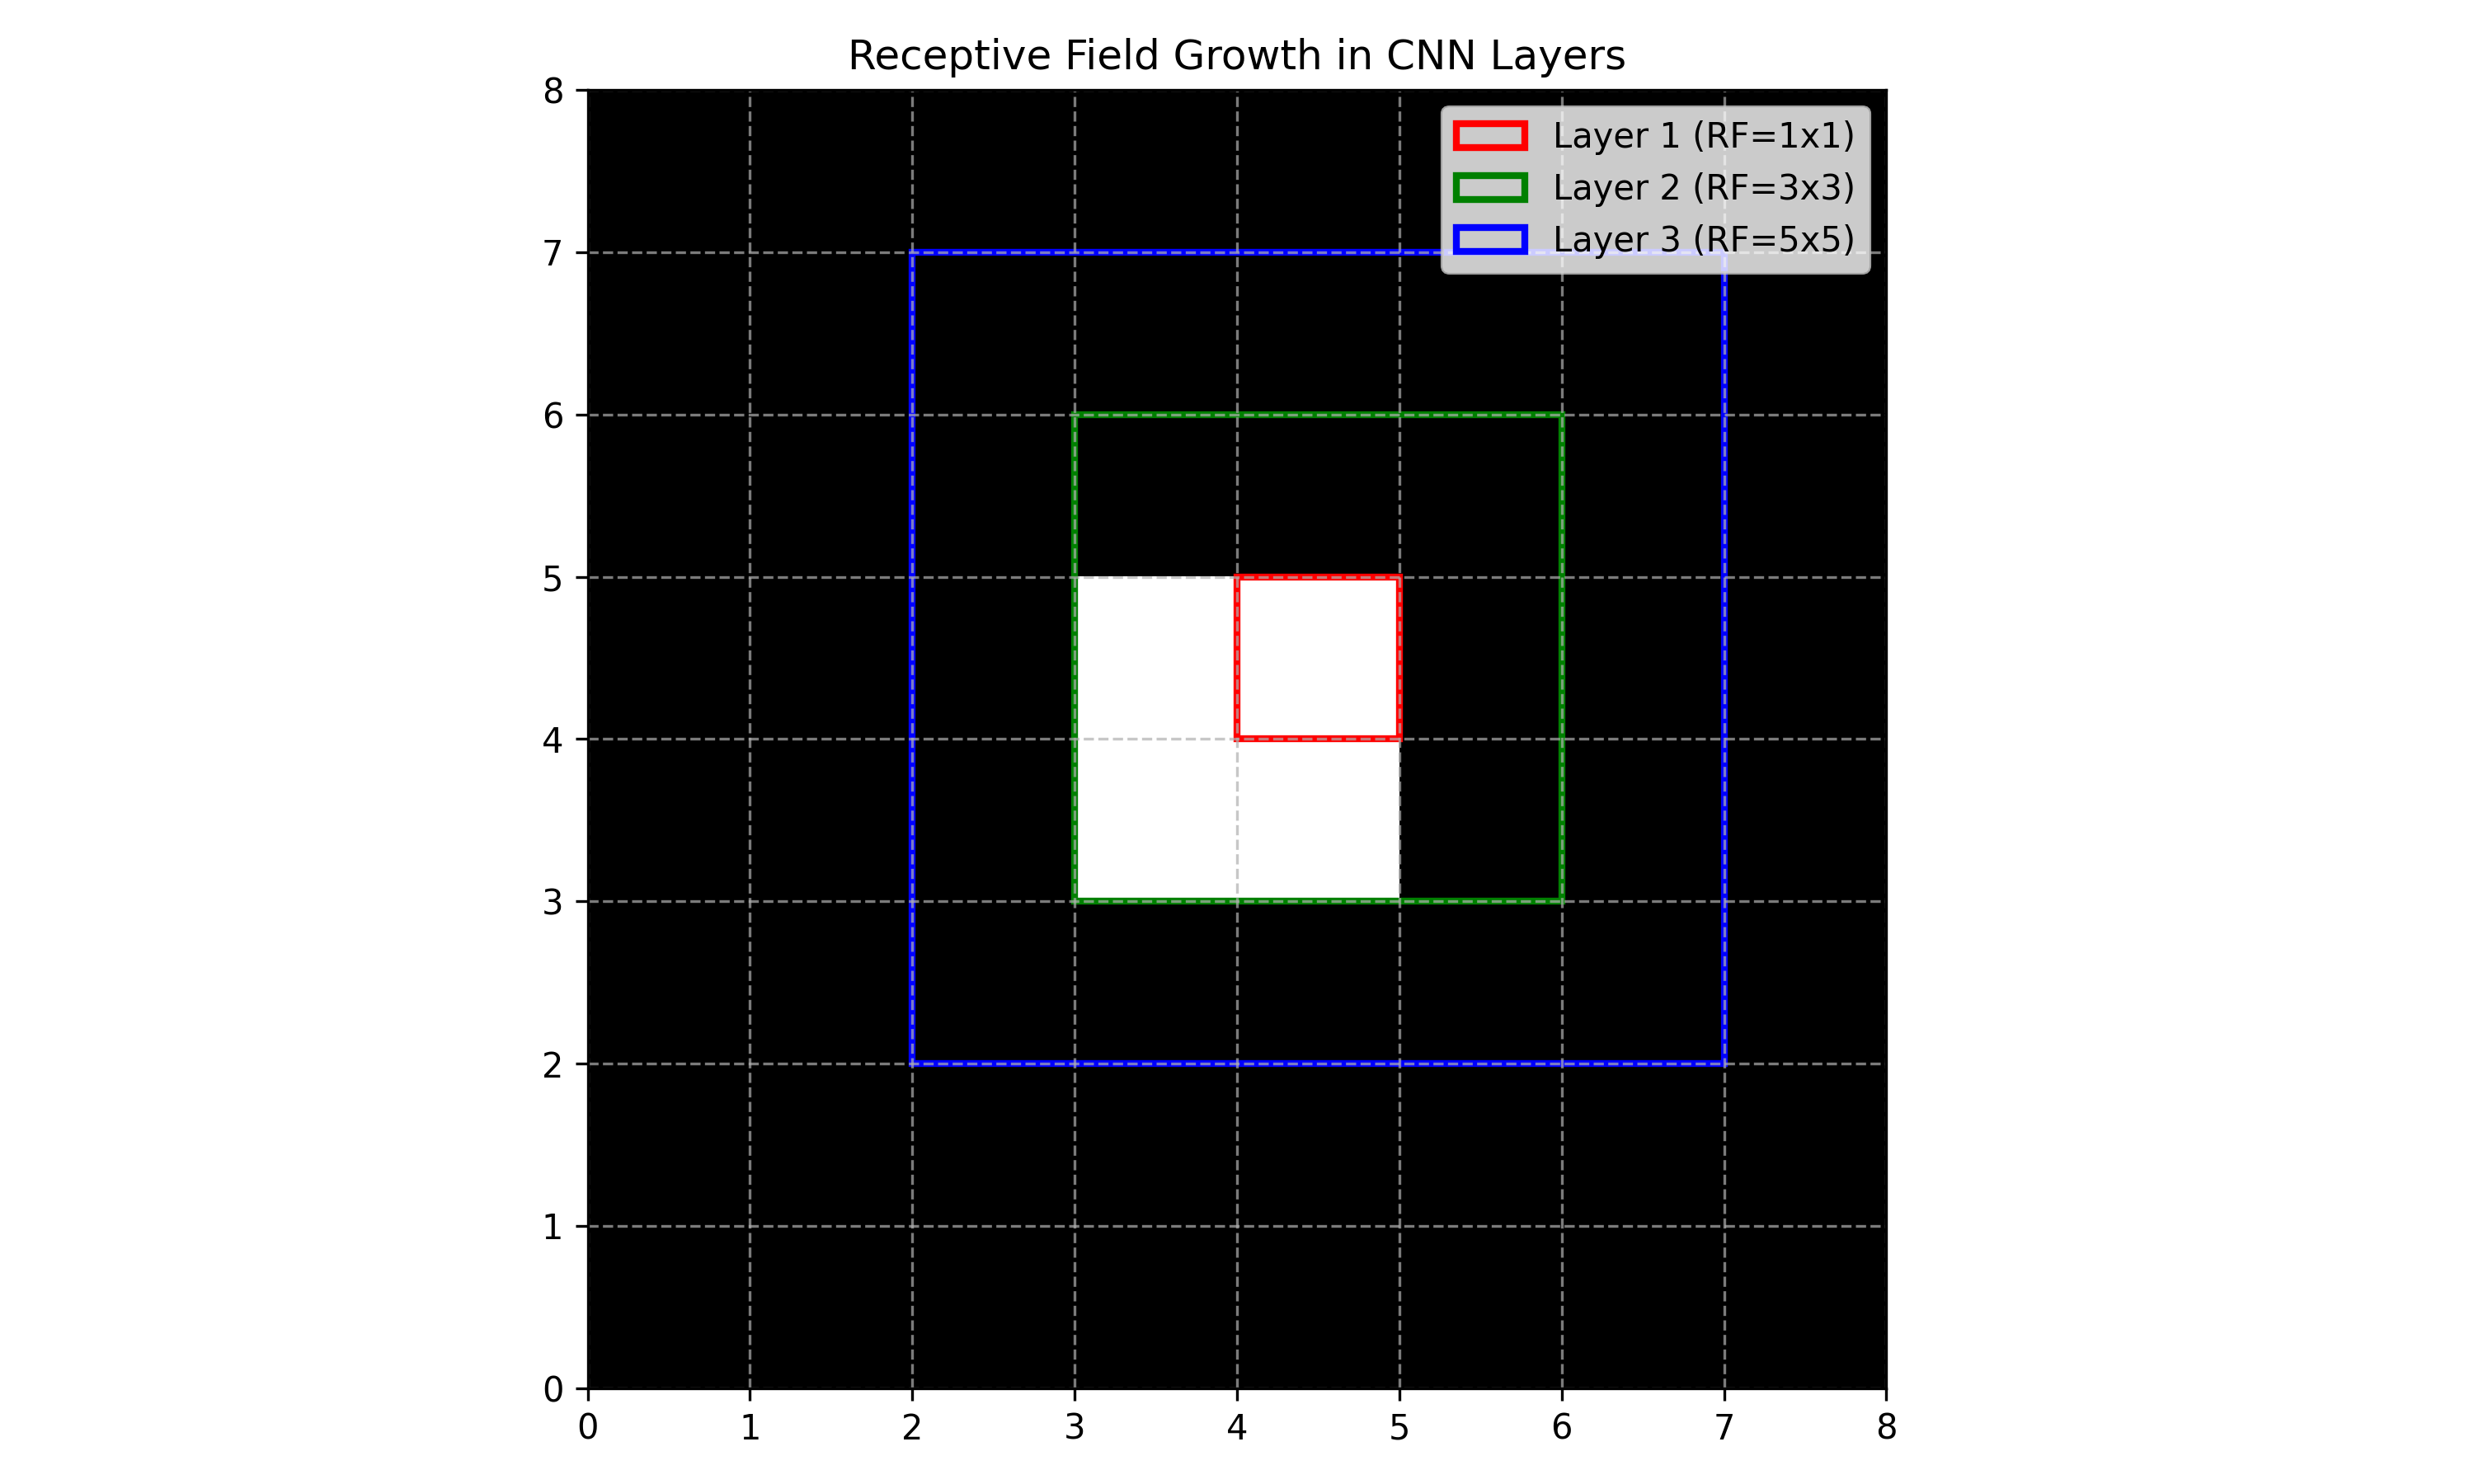
\includegraphics[width=0.8\textwidth]{Dissertation/images/receptive_field_diagram.png}
\caption{Пример расчета рецептивного поля через последовательные слои CNN. На каждом уровне область входа, влияющая на нейрон, увеличивается с учетом размера ядра и шага свертки.}
\label{fig:receptive_field_diagram}
\end{figure}

\subsection{Связь размера рецептивного поля с инвариантностью к сдвигу}
\label{theory:receptive_fields:shift_invariance}

Размер рецептивного поля имеет прямое отношение к способности CNN обеспечивать инвариантность к сдвигам различной величины. Интуитивно, чем больше рецептивное поле, тем более глобальные контекстные признаки может учитывать сеть при классификации или детекции, что потенциально способствует более стабильным предсказаниям при малых сдвигах объекта.

Однако важно отметить, что большое рецептивное поле само по себе не гарантирует инвариантность к сдвигу. Как показано в работах \cite{Zhang2019, Azulay2019}, даже CNN с крупными рецептивными полями могут демонстрировать значительную чувствительность к субпиксельным сдвигам, если не применяются специальные методы анти-алиасинга при даунсэмплинге.

Можно выделить следующие аспекты взаимосвязи между рецептивными полями и инвариантностью к сдвигу:

\begin{enumerate}
    \item \textbf{Верхняя граница инвариантности}: Нейрон не может быть инвариантен к сдвигам, превышающим размер его рецептивного поля, так как такие сдвиги выведут объект за пределы области, которую "видит" нейрон.
    
    \item \textbf{Кусочная инвариантность}: При достаточно больших рецептивных полях CNN может демонстрировать кусочную инвариантность — стабильность предсказаний в пределах определенных субрегионов входного пространства.
    
    \item \textbf{Чувствительность к границам рецептивного поля}: Эмпирически наблюдается повышенная чувствительность к сдвигам объектов, которые находятся на границах рецептивных полей критически важных нейронов.
    
    \item \textbf{Вложенные рецептивные поля}: Архитектуры с множеством параллельных путей и рецептивными полями разного размера (например, FPN в детекторах YOLO) часто демонстрируют лучшую инвариантность благодаря объединению признаков с разными масштабами и локальностью.
\end{enumerate}

\subsection{Эффективные рецептивные поля}
\label{theory:receptive_fields:effective}

Важно различать теоретическое рецептивное поле, рассчитанное по формуле выше, и эффективное рецептивное поле (ЭРП), которое характеризует область реального влияния на выход нейрона. Как показано в исследовании \cite{Luo2016}, эффективное рецептивное поле обычно меньше теоретического и имеет гауссовидную форму распределения влияния пикселей, с максимумом в центре.

В контексте инвариантности к сдвигу важны следующие свойства ЭРП:

\begin{itemize}
    \item \textbf{Центрированность}: Пиксели в центре ЭРП имеют наибольшее влияние на активацию нейрона.
    
    \item \textbf{Убывающее влияние}: Влияние пикселей уменьшается от центра к периферии, обычно по гауссовскому закону.
    
    \item \textbf{Зависимость от данных}: Размер и форма ЭРП могут варьироваться в зависимости от характеристик входных данных.
\end{itemize}

Таким образом, для достижения более высокой инвариантности к сдвигу желательно не только увеличивать теоретический размер рецептивного поля, но и учитывать особенности эффективного рецептивного поля, стремясь к более равномерному распределению влияния пикселей в его пределах.

В последующих разделах мы рассмотрим, как конкретные архитектуры CNN реализуют различные стратегии работы с рецептивными полями и как современные методы анти-алиасинга помогают улучшить инвариантность к сдвигу, воздействуя на характеристики этих полей.

\section{Описание архитектур CNN}
\label{theory:architectures}

В данном разделе мы опишем основные архитектуры CNN, используемые в наших экспериментах, и проанализируем их структурные особенности, влияющие на инвариантность к сдвигу.

\subsection{Архитектура VGG}
\label{theory:architectures:vgg}

Архитектура VGG, предложенная Симоняном и Зиссерманом \cite{Simonyan2015}, является одной из классических архитектур глубоких CNN. Её главная особенность — использование однородных сверточных слоев с малыми ядрами размера 3×3 и максимальным пулингом с окном 2×2 и шагом 2 для понижения пространственного разрешения.

\begin{figure}[ht]
\centering
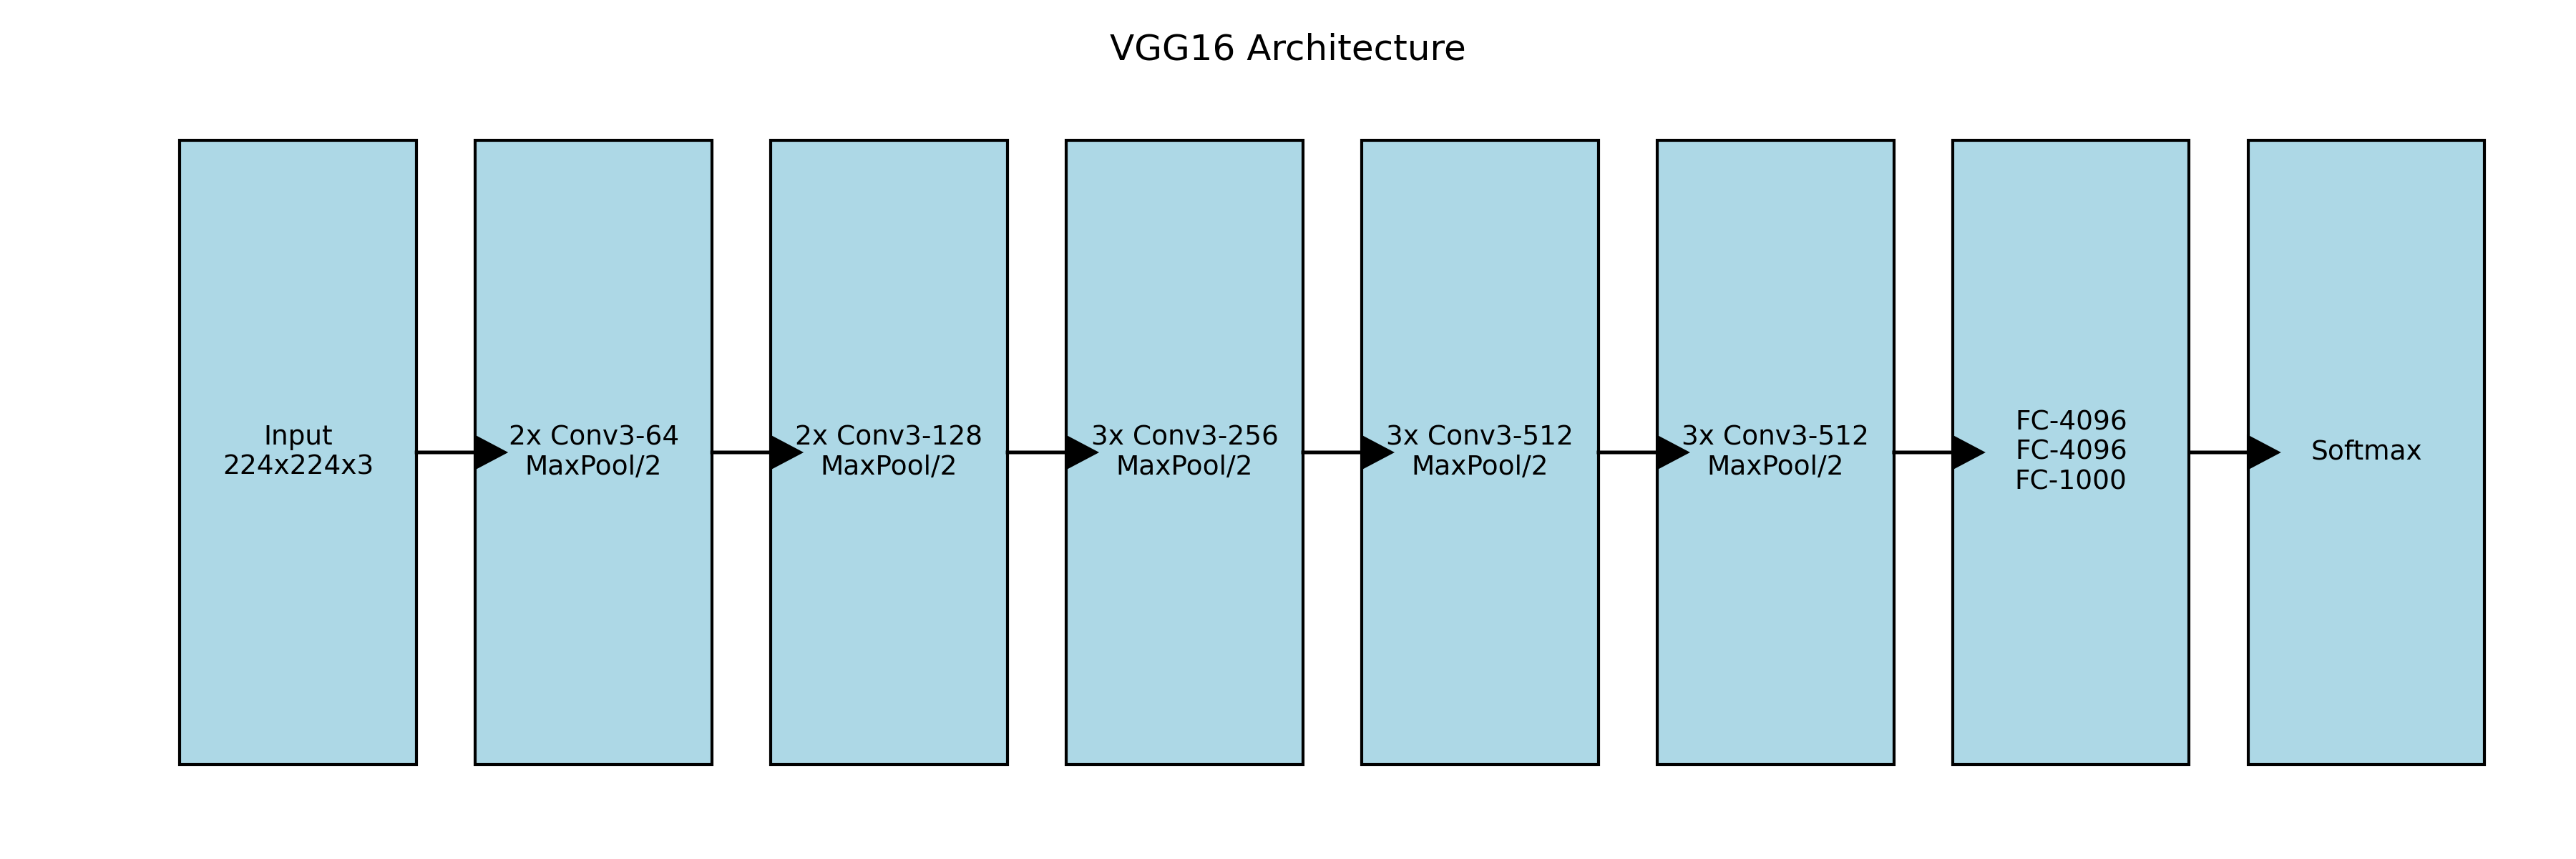
\includegraphics[width=0.9\textwidth]{Dissertation/images/vgg16_architecture.png}
\caption{Архитектура VGG16. Сеть состоит из 13 сверточных слоев с малыми ядрами 3×3 и 3 полносвязных слоев. Пространственное разрешение уменьшается с помощью операций максимального пулинга (max pooling) с шагом 2.}
\label{fig:vgg16_architecture}
\end{figure}

Структура VGG16 включает 5 блоков со сверточными слоями, разделенными слоями пулинга, и завершается тремя полносвязными слоями (рис. \ref{fig:vgg16_architecture}). Каждый сверточный слой сопровождается нелинейной функцией активации ReLU.

В контексте пространственной инвариантности VGG имеет следующие характеристики:

\begin{itemize}
    \item \textbf{Рецептивное поле}: Теоретическое рецептивное поле конечных слоев VGG16 составляет 212×212 пикселей, что достаточно велико для захвата глобальных признаков изображения.
    
    \item \textbf{Даунсэмплинг}: VGG использует 5 операций максимального пулинга, что приводит к общему коэффициенту понижения разрешения $2^5 = 32$. Это означает, что выходная карта признаков в последнем сверточном слое имеет разрешение в 32 раза меньше, чем входное изображение.
    
    \item \textbf{Чувствительность к сдвигу}: Из-за использования операций максимального пулинга без сглаживания, VGG склонна к проблемам алиасинга, что делает её особенно чувствительной к малым сдвигам входных данных.
\end{itemize}

Регулярная структура VGG делает её удобной моделью для изучения эффектов анти-алиасинга и модификации для улучшения инвариантности к сдвигу.

\subsection{Архитектура ResNet}
\label{theory:architectures:resnet}

Архитектура ResNet (Residual Network), предложенная He и др. \cite{He2016}, ввела концепцию остаточных соединений для решения проблемы затухания градиентов в очень глубоких сетях. Ключевой компонент ResNet — остаточный блок, который добавляет результат «обходного» соединения к выходу стека сверточных слоев.

\begin{figure}[ht]
\centering
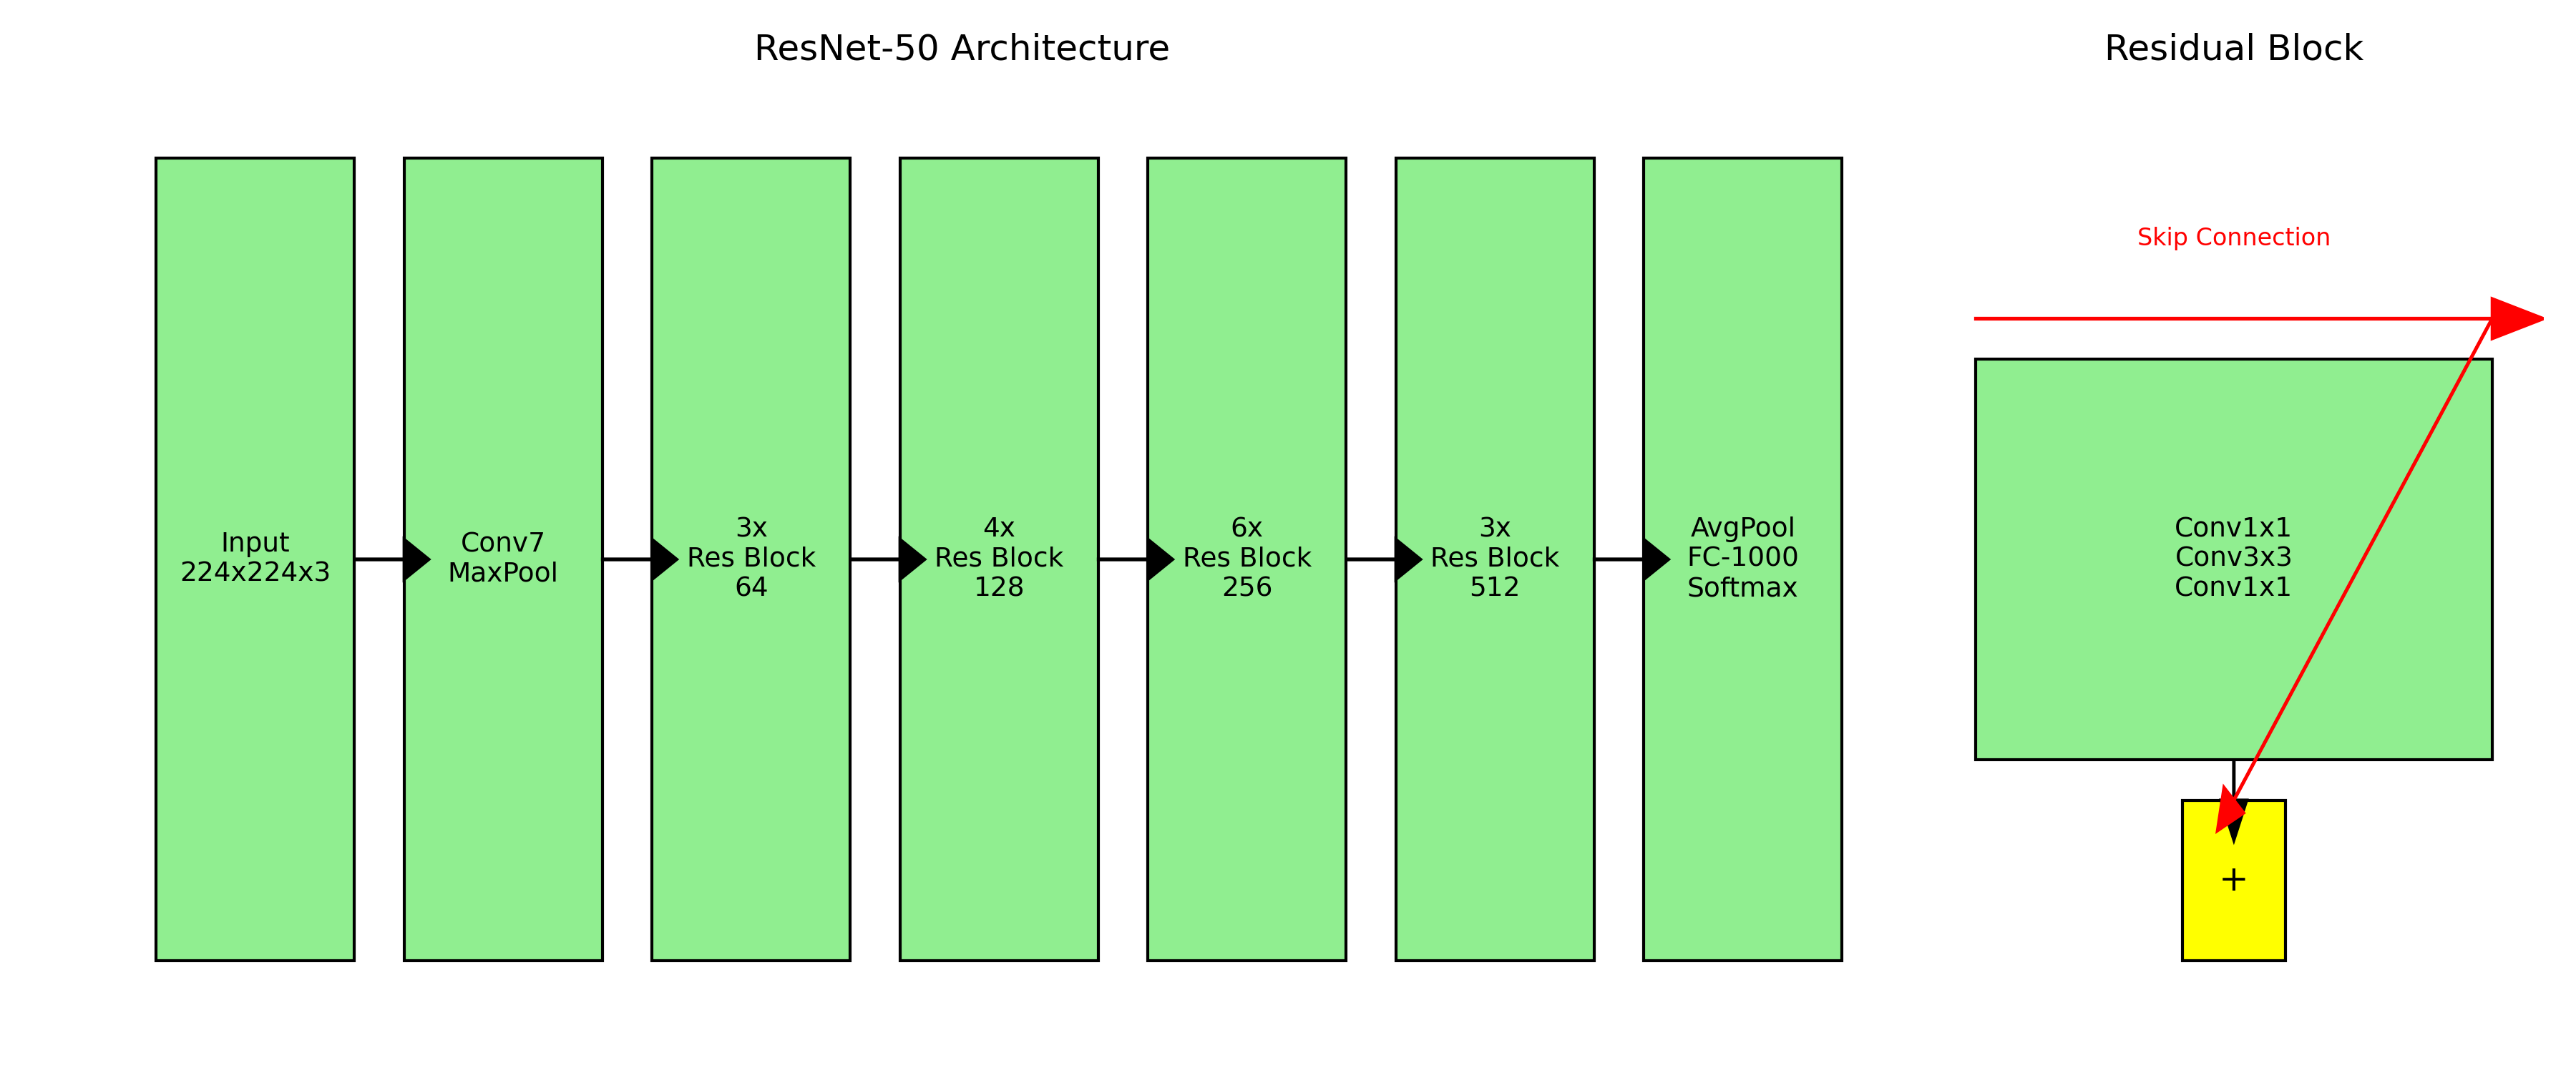
\includegraphics[width=0.9\textwidth]{Dissertation/images/resnet_architecture.png}
\caption{Архитектура ResNet. Слева: общая структура ResNet-50. Справа: детализация остаточного блока с обходным соединением, позволяющим информации напрямую проходить между слоями.}
\label{fig:resnet_architecture}
\end{figure}

В наших экспериментах используется ResNet-50, которая включает начальный сверточный слой с ядром 7×7 и шагом 2, за которым следует слой максимального пулинга с размером окна 3×3 и шагом 2, а затем 4 каскада остаточных блоков (рис. \ref{fig:resnet_architecture}). Пространственное разрешение уменьшается в начале каждого каскада (кроме первого) с использованием свертки с шагом 2.

С точки зрения пространственной инвариантности ResNet характеризуется следующими особенностями:

\begin{itemize}
    \item \textbf{Рецептивное поле}: ResNet-50 имеет теоретическое рецептивное поле размером 483×483 пикселя, что значительно больше, чем у VGG16.
    
    \item \textbf{Даунсэмплинг}: ResNet использует комбинацию свертки с шагом 2 и максимального пулинга для даунсэмплинга, с общим коэффициентом понижения разрешения 32, аналогично VGG.
    
    \item \textbf{Остаточные соединения}: Обходные соединения в ResNet позволяют информации «перепрыгивать» через слои даунсэмплинга, что потенциально может помочь сохранить некоторые аспекты пространственной информации.
    
    \item \textbf{Свёртка с шагом}: В отличие от VGG, которая использует исключительно максимальный пулинг для даунсэмплинга, ResNet также применяет свертку с шагом 2, что создает другой профиль чувствительности к алиасингу.
\end{itemize}

Эмпирически было показано, что архитектуры типа ResNet несколько более устойчивы к малым сдвигам, чем VGG, что может быть связано с использованием остаточных соединений и меньшим количеством операций максимального пулинга.

\subsection{Архитектура YOLO}
\label{theory:architectures:yolo}

YOLO (You Only Look Once) — семейство моделей для детекции объектов, предложенное Redmon и др. \cite{Redmon2016}. В отличие от VGG и ResNet, которые преимущественно используются для классификации, YOLO предназначена для одновременного определения местоположения объектов и их классификации. В наших экспериментах используется YOLOv5s, современная реализация архитектуры YOLO.

\begin{figure}[ht]
\centering
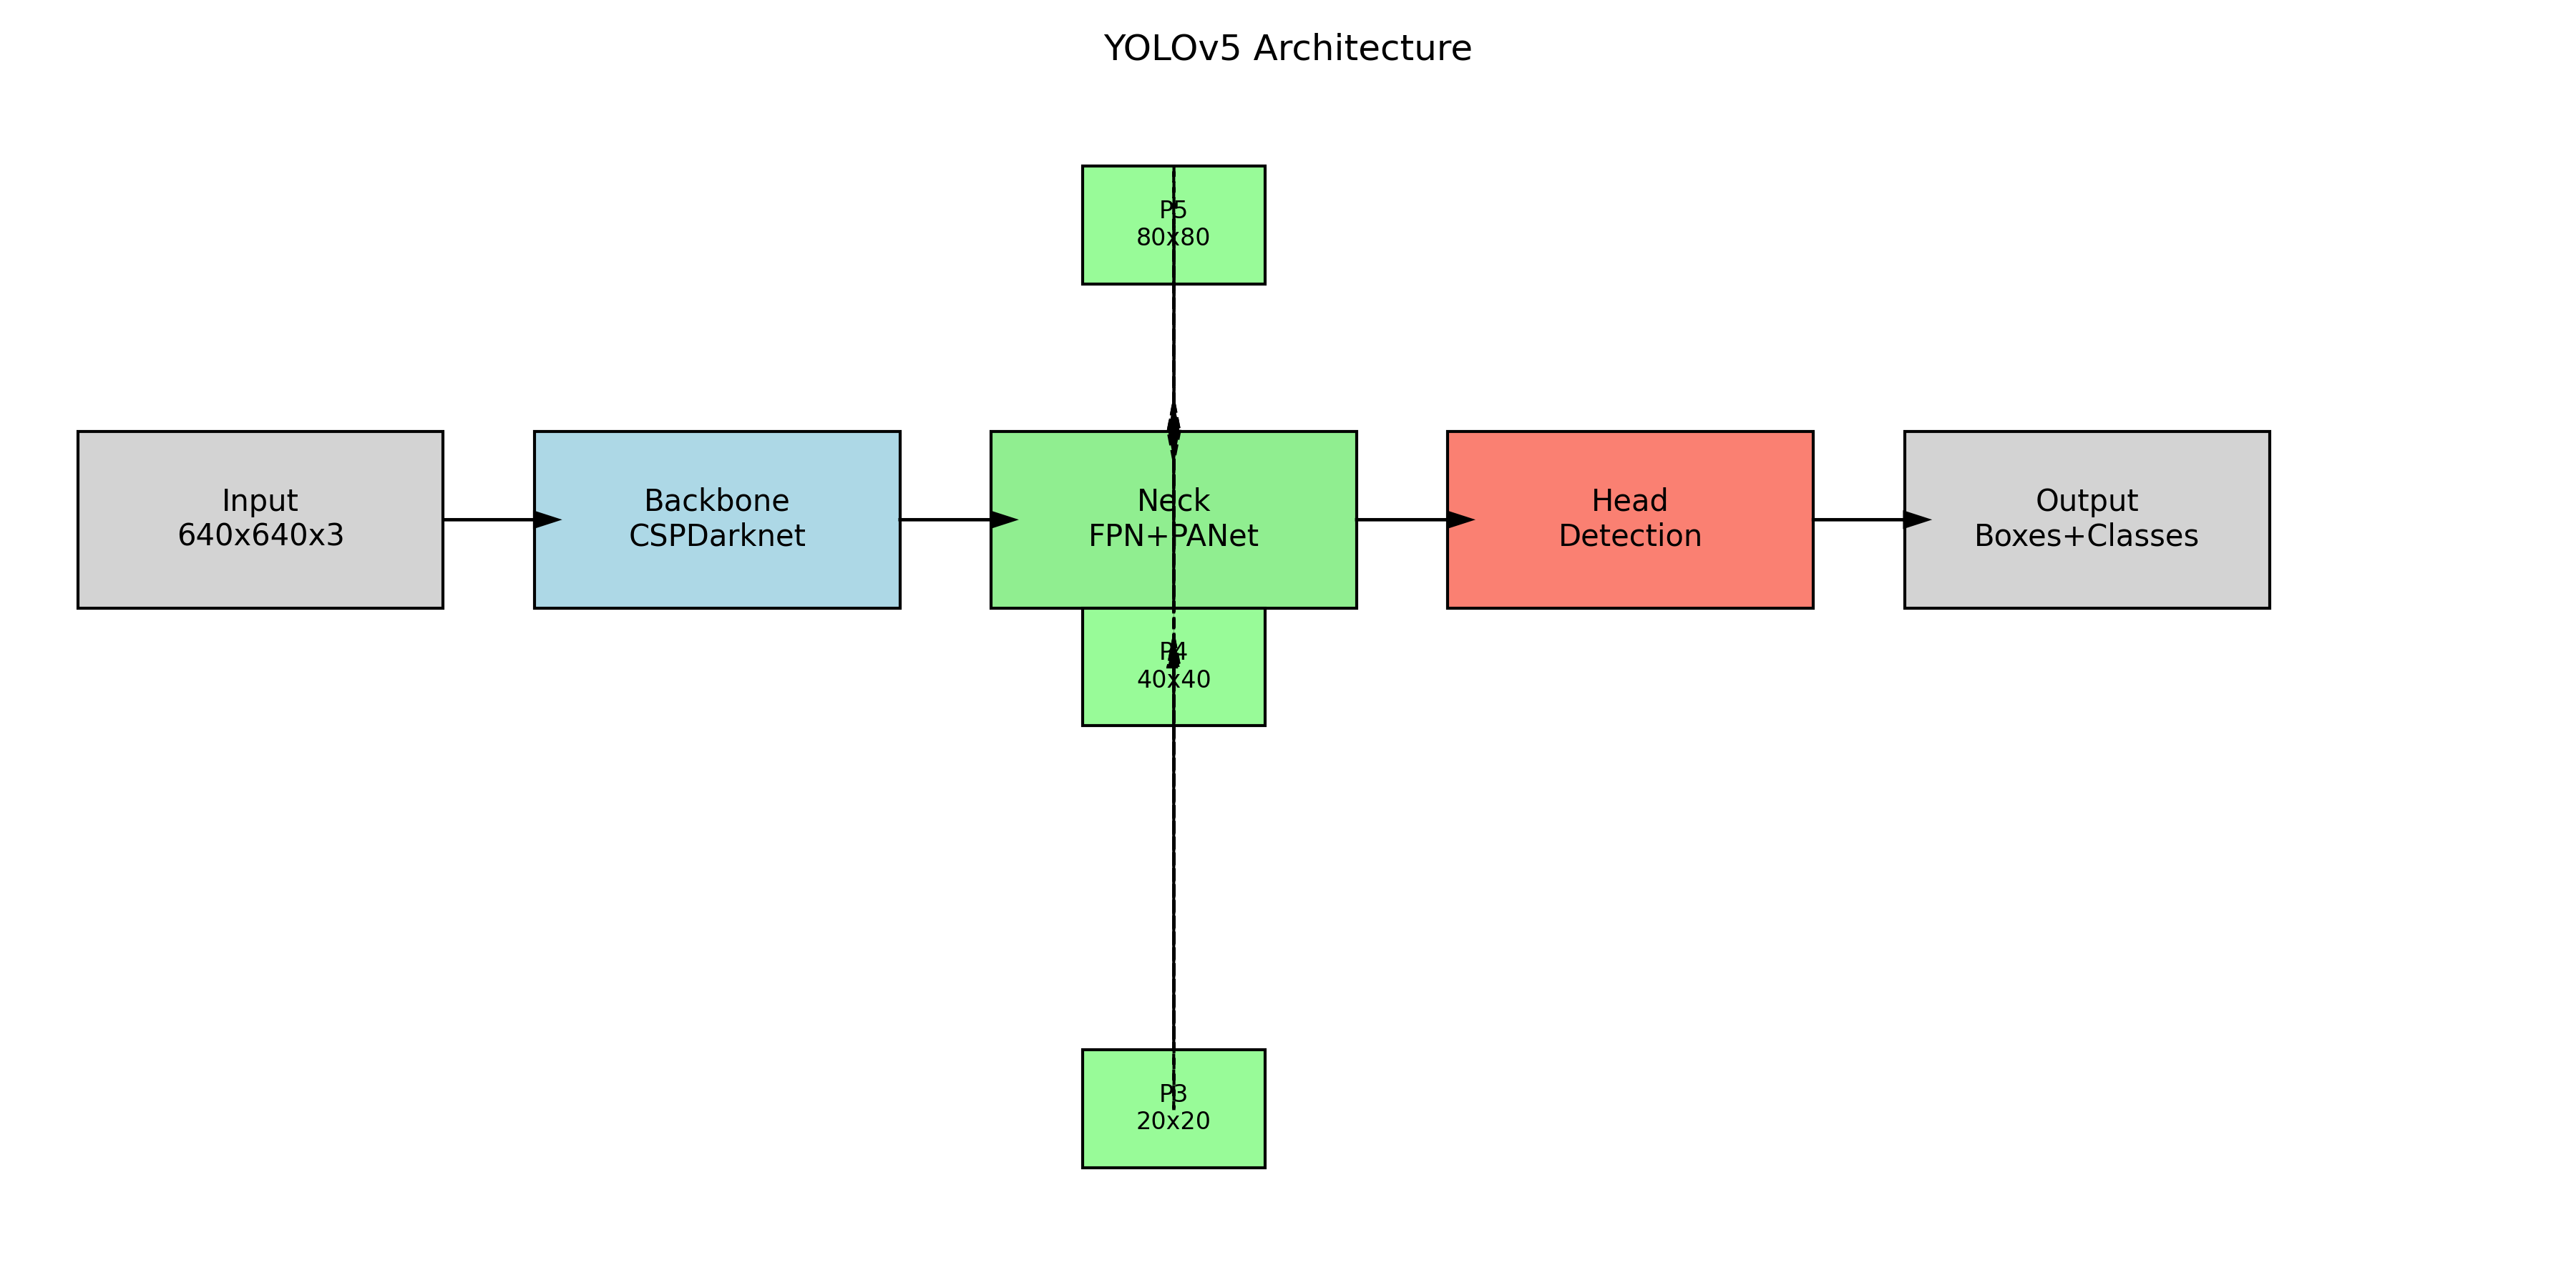
\includegraphics[width=\textwidth]{Dissertation/images/yolov5_architecture.png}
\caption{Архитектура YOLOv5. Сеть включает (а) магистральную часть (backbone) для извлечения признаков, (б) шею (neck) с пирамидой признаков FPN для объединения информации с разных масштабов, и (в) голову (head) для предсказания ограничивающих рамок и классов объектов.}
\label{fig:yolov5_architecture}
\end{figure}

Архитектура YOLOv5 (рис. \ref{fig:yolov5_architecture}) состоит из трех основных компонентов:

\begin{enumerate}
    \item \textbf{Backbone (магистраль)}: CSPDarknet, состоящий из модулей Cross Stage Partial (CSP), для эффективного извлечения признаков.
    
    \item \textbf{Neck (шея)}: Пирамида признаков (FPN) с дополнительными обходными соединениями (PANet), которая объединяет информацию с разных уровней детализации.
    
    \item \textbf{Head (голова)}: Сеть предсказания, которая выдает ограничивающие рамки, вероятности наличия объекта и вероятности классов.
\end{enumerate}

Особенности YOLOv5 с точки зрения пространственной инвариантности:

\begin{itemize}
    \item \textbf{Многомасштабные предсказания}: YOLOv5 выполняет предсказания на трех разных масштабах (уровнях пирамиды признаков), что теоретически должно повышать устойчивость к малым смещениям объектов.
    
    \item \textbf{Рецептивные поля разного размера}: Благодаря архитектуре FPN/PANet, YOLOv5 объединяет информацию из рецептивных полей разного размера, что может помогать в достижении более стабильных предсказаний.
    
    \item \textbf{Даунсэмплинг}: YOLOv5 использует максимальный пулинг и свертку с шагом 2 для понижения пространственного разрешения, что делает её потенциально чувствительной к проблемам алиасинга, аналогично VGG и ResNet.
    
    \item \textbf{Предсказание смещений}: YOLO предсказывает не абсолютные координаты ограничивающих рамок, а смещения относительно опорных рамок (anchors), что влияет на чувствительность к пространственным сдвигам.
\end{itemize}

\subsection{Сравнение архитектур с точки зрения пространственной инвариантности}
\label{theory:architectures:comparison}

Обобщим ключевые характеристики рассмотренных архитектур в контексте их потенциальной инвариантности к пространственным сдвигам:

\begin{table}[ht]
\centering
\caption{Сравнение архитектур CNN с точки зрения характеристик, влияющих на пространственную инвариантность}
\label{tab:architecture_comparison}
\begin{tabular}{|l|c|c|c|c|}
\hline
\textbf{Архитектура} & \textbf{Рецептивное поле} & \textbf{Даунсэмплинг} & \textbf{Метод даунсэмплинга} & \textbf{Особенности} \\ \hline
VGG16 & 212×212 & 32× & Max pooling & Однородные слои \\ \hline
ResNet-50 & 483×483 & 32× & Stride conv + max pooling & Остаточные соединения \\ \hline
YOLOv5s & $\sim$725×725 & 32× & Stride conv + max pooling & Многомасштабные предсказания \\ \hline
\end{tabular}
\end{table}

Как видно из таблицы \ref{tab:architecture_comparison}, все три архитектуры используют даунсэмплинг с коэффициентом 32, но различаются по методам его реализации и размеру рецептивного поля. Эти различия, а также специфические архитектурные особенности каждой модели, влияют на их чувствительность к субпиксельным сдвигам входных изображений.

В экспериментальной части работы мы количественно оценим степень пространственной инвариантности каждой из этих архитектур и проанализируем, как различные модификации, в частности методы анти-алиасинга, влияют на эту характеристику.

\section{Теория анти-алиасинга в CNN}
\label{theory:anti_aliasing}

В данном разделе мы подробно рассмотрим причины возникновения проблемы алиасинга в CNN и методы её решения, в частности, технологии BlurPool и TIPS, которые используются в наших экспериментах.

\subsection{Причины алиасинга в операциях даунсэмплинга}
\label{theory:anti_aliasing:causes}

Даунсэмплинг (понижение пространственного разрешения) является неотъемлемой частью современных CNN, позволяя увеличивать рецептивное поле и уменьшать вычислительную сложность. Однако эти операции создают проблему алиасинга, которая негативно влияет на инвариантность к сдвигу.

\begin{figure}[ht]
\centering
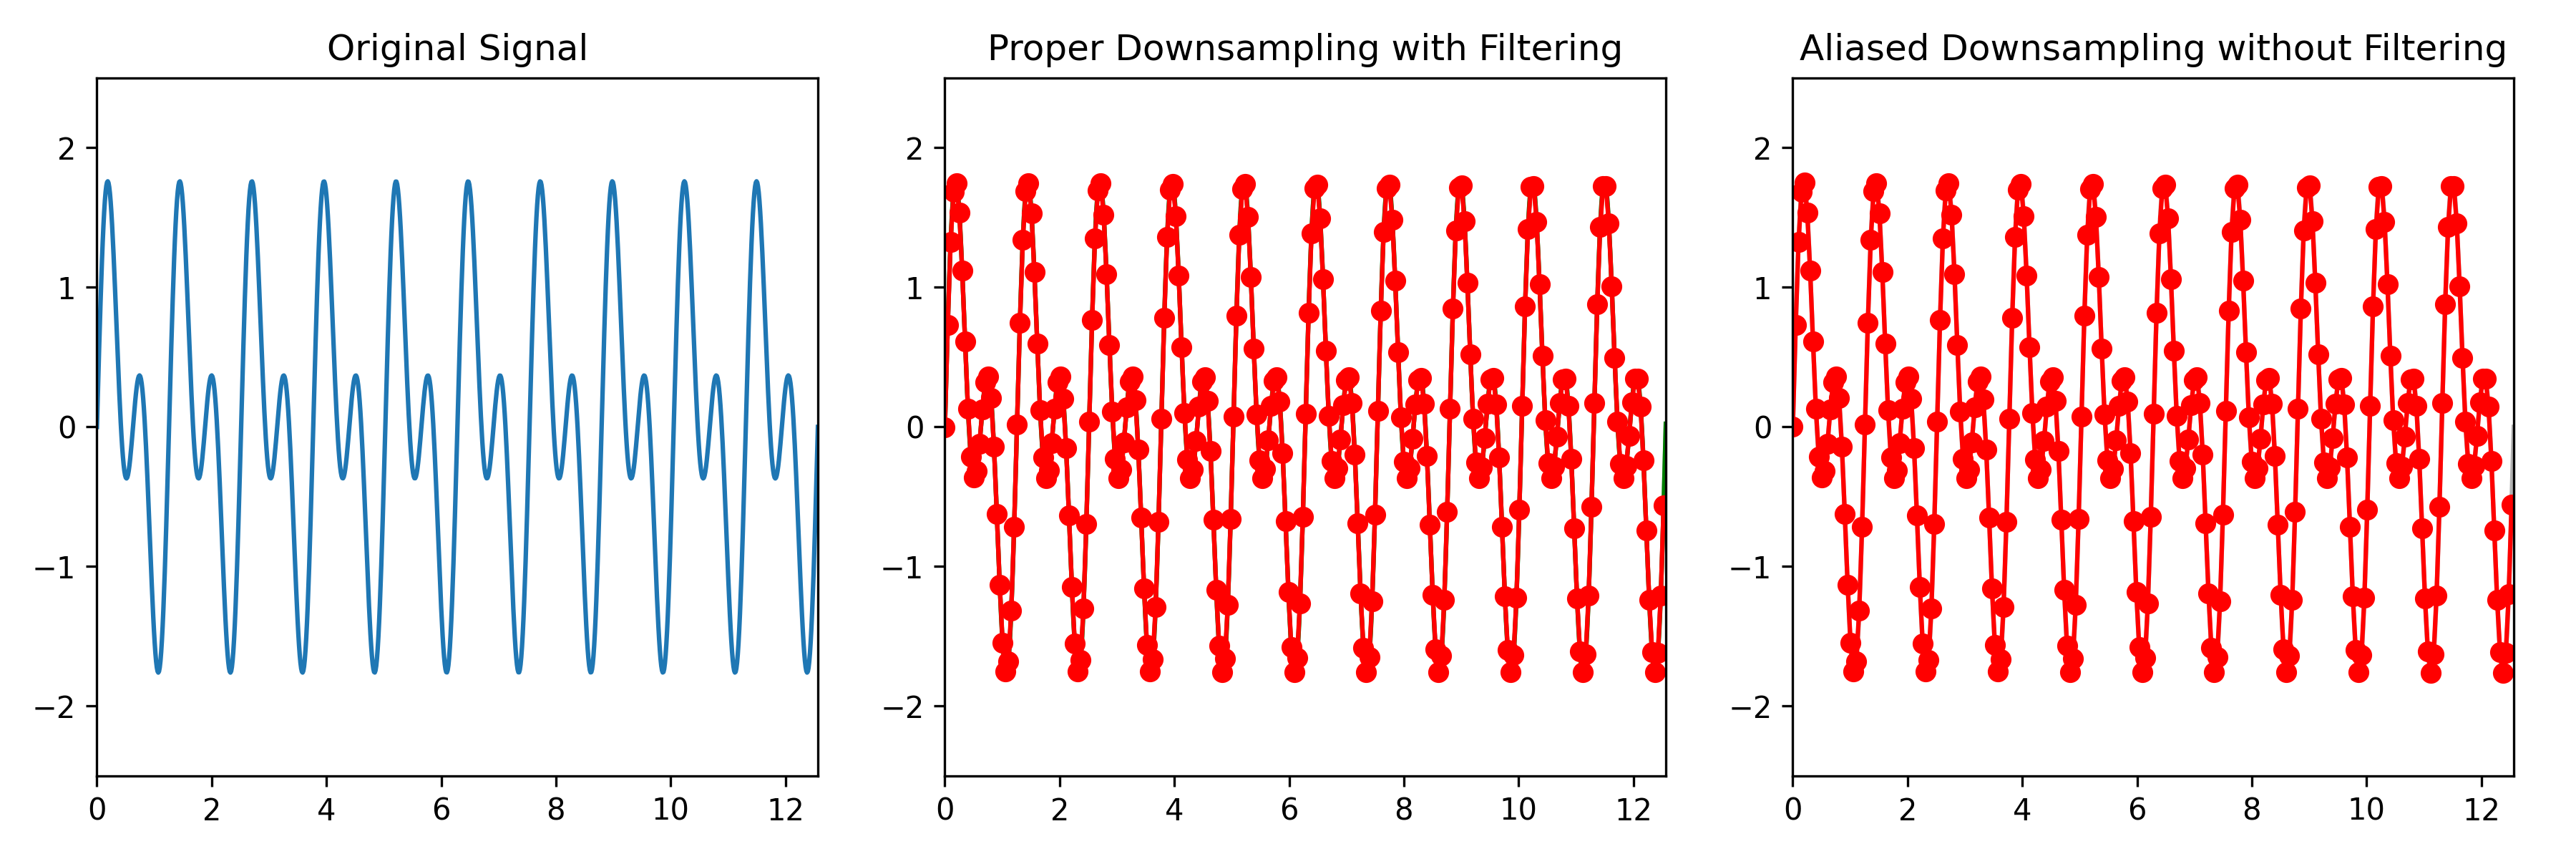
\includegraphics[width=0.8\textwidth]{Dissertation/images/aliasing_example.png}
\caption{Пример алиасинга при даунсэмплинге: слева — оригинальный сигнал, в центре — корректный даунсэмплинг с предварительной фильтрацией, справа — даунсэмплинг без фильтрации, приводящий к алиасингу.}
\label{fig:aliasing_example}
\end{figure}

Алиасинг возникает, когда высокочастотные компоненты сигнала (в нашем случае — карты признаков) недостаточно отфильтрованы перед понижением частоты дискретизации (рис. \ref{fig:aliasing_example}). Согласно теореме Найквиста-Шеннона, для корректного представления сигнала частота дискретизации должна быть как минимум вдвое выше максимальной частоты в сигнале. При даунсэмплинге частота дискретизации уменьшается, что может привести к "складыванию" высоких частот в низкие (алиасингу), если не применить предварительную низкочастотную фильтрацию.

В классических CNN используются два основных метода даунсэмплинга:

\begin{itemize}
    \item \textbf{Максимальный пулинг}: Выбор максимального значения в каждом окне размера $k \times k$ с шагом $s$. Операция не линейна и не обладает анти-алиасинговыми свойствами.
    
    \item \textbf{Свёртка с шагом (strided convolution)}: Применение сверточного фильтра с шагом $s > 1$. Обеспечивает некоторую фильтрацию, но обычно недостаточную для предотвращения алиасинга.
\end{itemize}

Математически проблему алиасинга можно представить следующим образом. Пусть $X[n,m]$ — дискретная карта признаков, а $X_d[n,m] = X[sn, sm]$ — результат даунсэмплинга с шагом $s$. В частотной области:

\begin{equation}
X_d(e^{j\omega_1}, e^{j\omega_2}) = \frac{1}{s^2} \sum_{k=0}^{s-1} \sum_{l=0}^{s-1} X(e^{j(\omega_1 - 2\pi k)/s}, e^{j(\omega_2 - 2\pi l)/s})
\end{equation}

где происходит наложение копий спектра, что и создает эффект алиасинга.

\subsection{Метод BlurPool}
\label{theory:anti_aliasing:blurpool}

Метод BlurPool, предложенный Zhang \cite{Zhang2019}, основан на классическом подходе обработки сигналов: перед понижением частоты дискретизации необходимо применить низкочастотный фильтр (НЧФ) для удаления высоких частот, которые могут вызвать алиасинг.

\begin{figure}[ht]
\centering
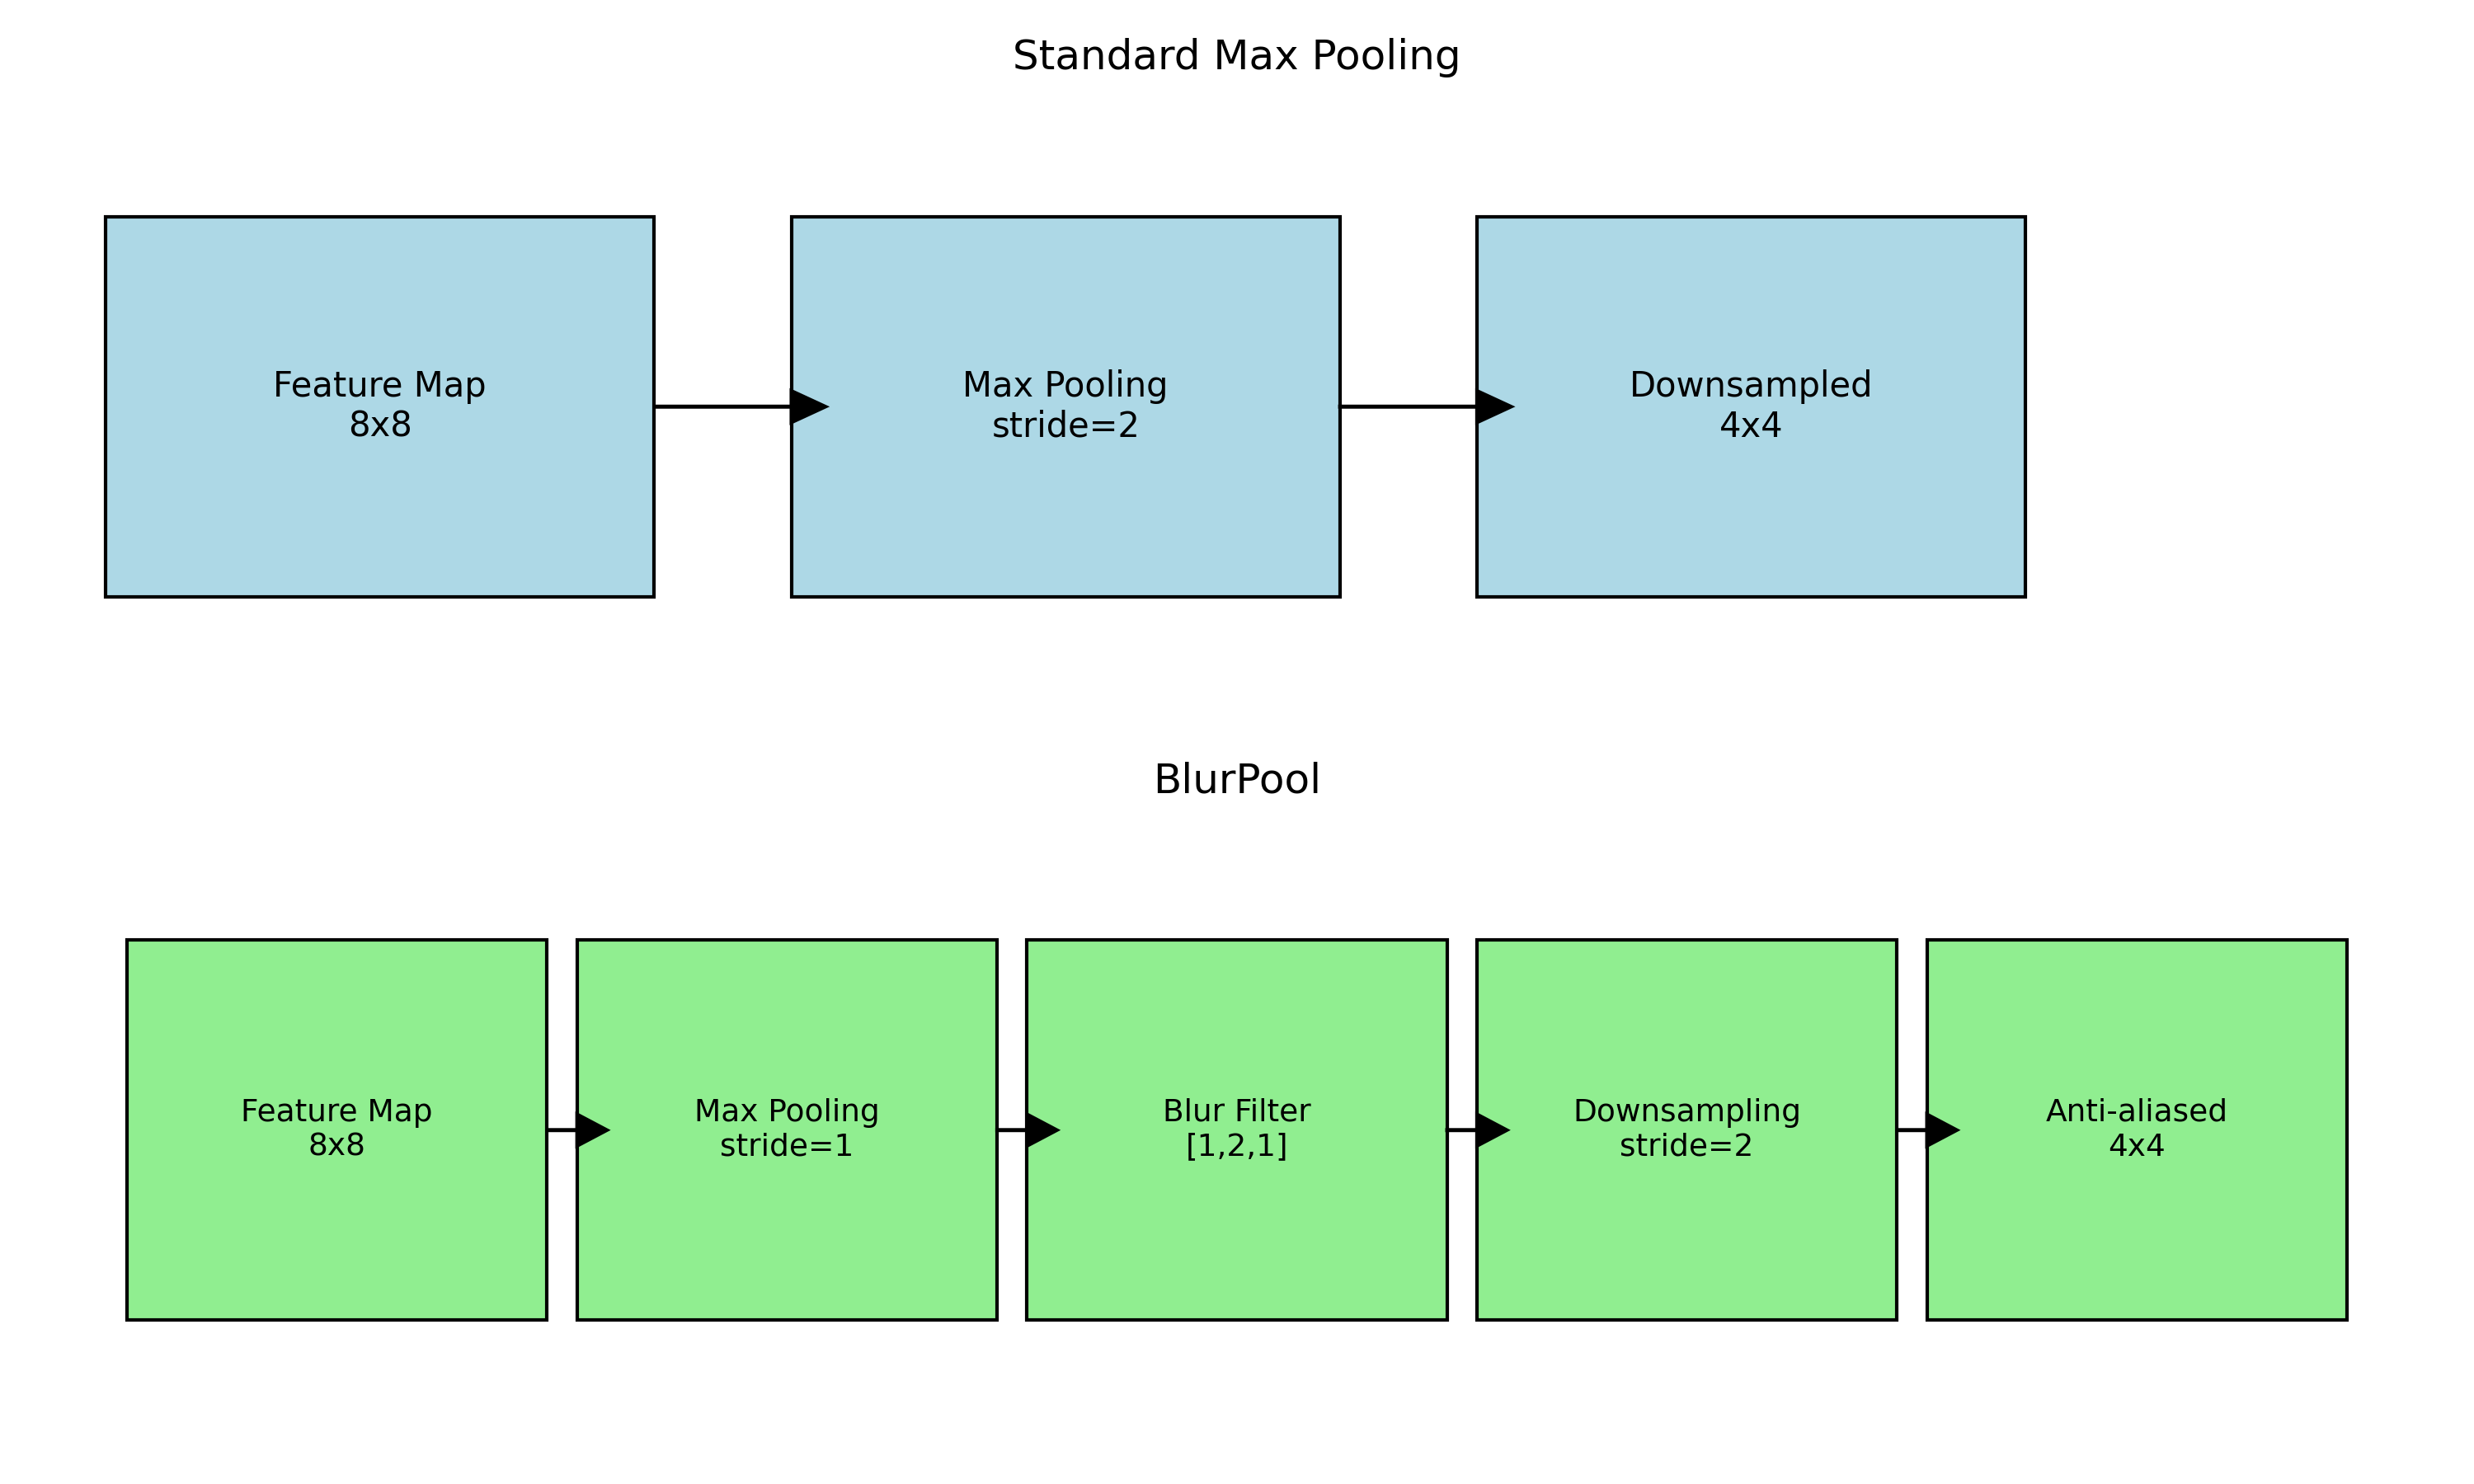
\includegraphics[width=0.8\textwidth]{Dissertation/images/blurpool_illustration.png}
\caption{Принцип работы BlurPool: вместо стандартной операции максимального пулинга (сверху) используется последовательность из максимального пулинга, размытия и даунсэмплинга (снизу).}
\label{fig:blurpool_illustration}
\end{figure}

Реализация BlurPool заключается в следующем:

\begin{enumerate}
    \item Применение низкочастотного фильтра к карте признаков для сглаживания высоких частот.
    \item Выполнение операции даунсэмплинга (с шагом $s$).
\end{enumerate}

В качестве низкочастотного фильтра Zhang предлагает использовать 2D фильтры, полученные как тензорное произведение одномерных биномиальных фильтров различного порядка:

\begin{itemize}
    \item Фильтр 1-го порядка: $[1, 1]$ (нормализованный как $[0.5, 0.5]$)
    \item Фильтр 2-го порядка: $[1, 2, 1]$ (нормализованный как $[0.25, 0.5, 0.25]$)
    \item Фильтр 3-го порядка: $[1, 3, 3, 1]$ (нормализованный как $[0.125, 0.375, 0.375, 0.125]$)
    \item Фильтр 4-го порядка: $[1, 4, 6, 4, 1]$ (нормализованный как $[0.0625, 0.25, 0.375, 0.25, 0.0625]$)
\end{itemize}

Двумерный фильтр размера $k \times k$ формируется как:

\begin{equation}
F_{2D}[n,m] = F_{1D}[n] \cdot F_{1D}[m]
\end{equation}

где $F_{1D}$ — одномерный биномиальный фильтр.

Применение BlurPool в сверточных нейронных сетях возможно несколькими способами:

\begin{enumerate}
    \item \textbf{Замена максимального пулинга}: Вместо операции максимального пулинга используется последовательность из максимального пулинга без шага (stride=1), затем блока размытия и даунсэмплинга.
    
    \item \textbf{Модификация свертки с шагом}: После сверточного слоя с шагом $s > 1$ добавляется дополнительная свертка с НЧФ и шагом 1, либо сам сверточный фильтр предварительно модифицируется для включения НЧФ.
\end{enumerate}

Экспериментально показано, что BlurPool значительно улучшает инвариантность CNN к сдвигам, особенно в случае замены операций максимального пулинга, которые являются основным источником алиасинга в сетях типа VGG.

\subsection{Метод TIPS}
\label{theory:anti_aliasing:tips}

TIPS (Translation Invariant Polyphase Sampling), предложенный Chaman и Dokmanić \cite{Chaman2021}, представляет собой более теоретически обоснованный подход к проблеме алиасинга в CNN. В отличие от BlurPool, который применяет фиксированные фильтры, TIPS использует полифазное представление сигнала и адаптирует фильтрацию в зависимости от конкретного субпиксельного сдвига.

\begin{figure}[ht]
\centering
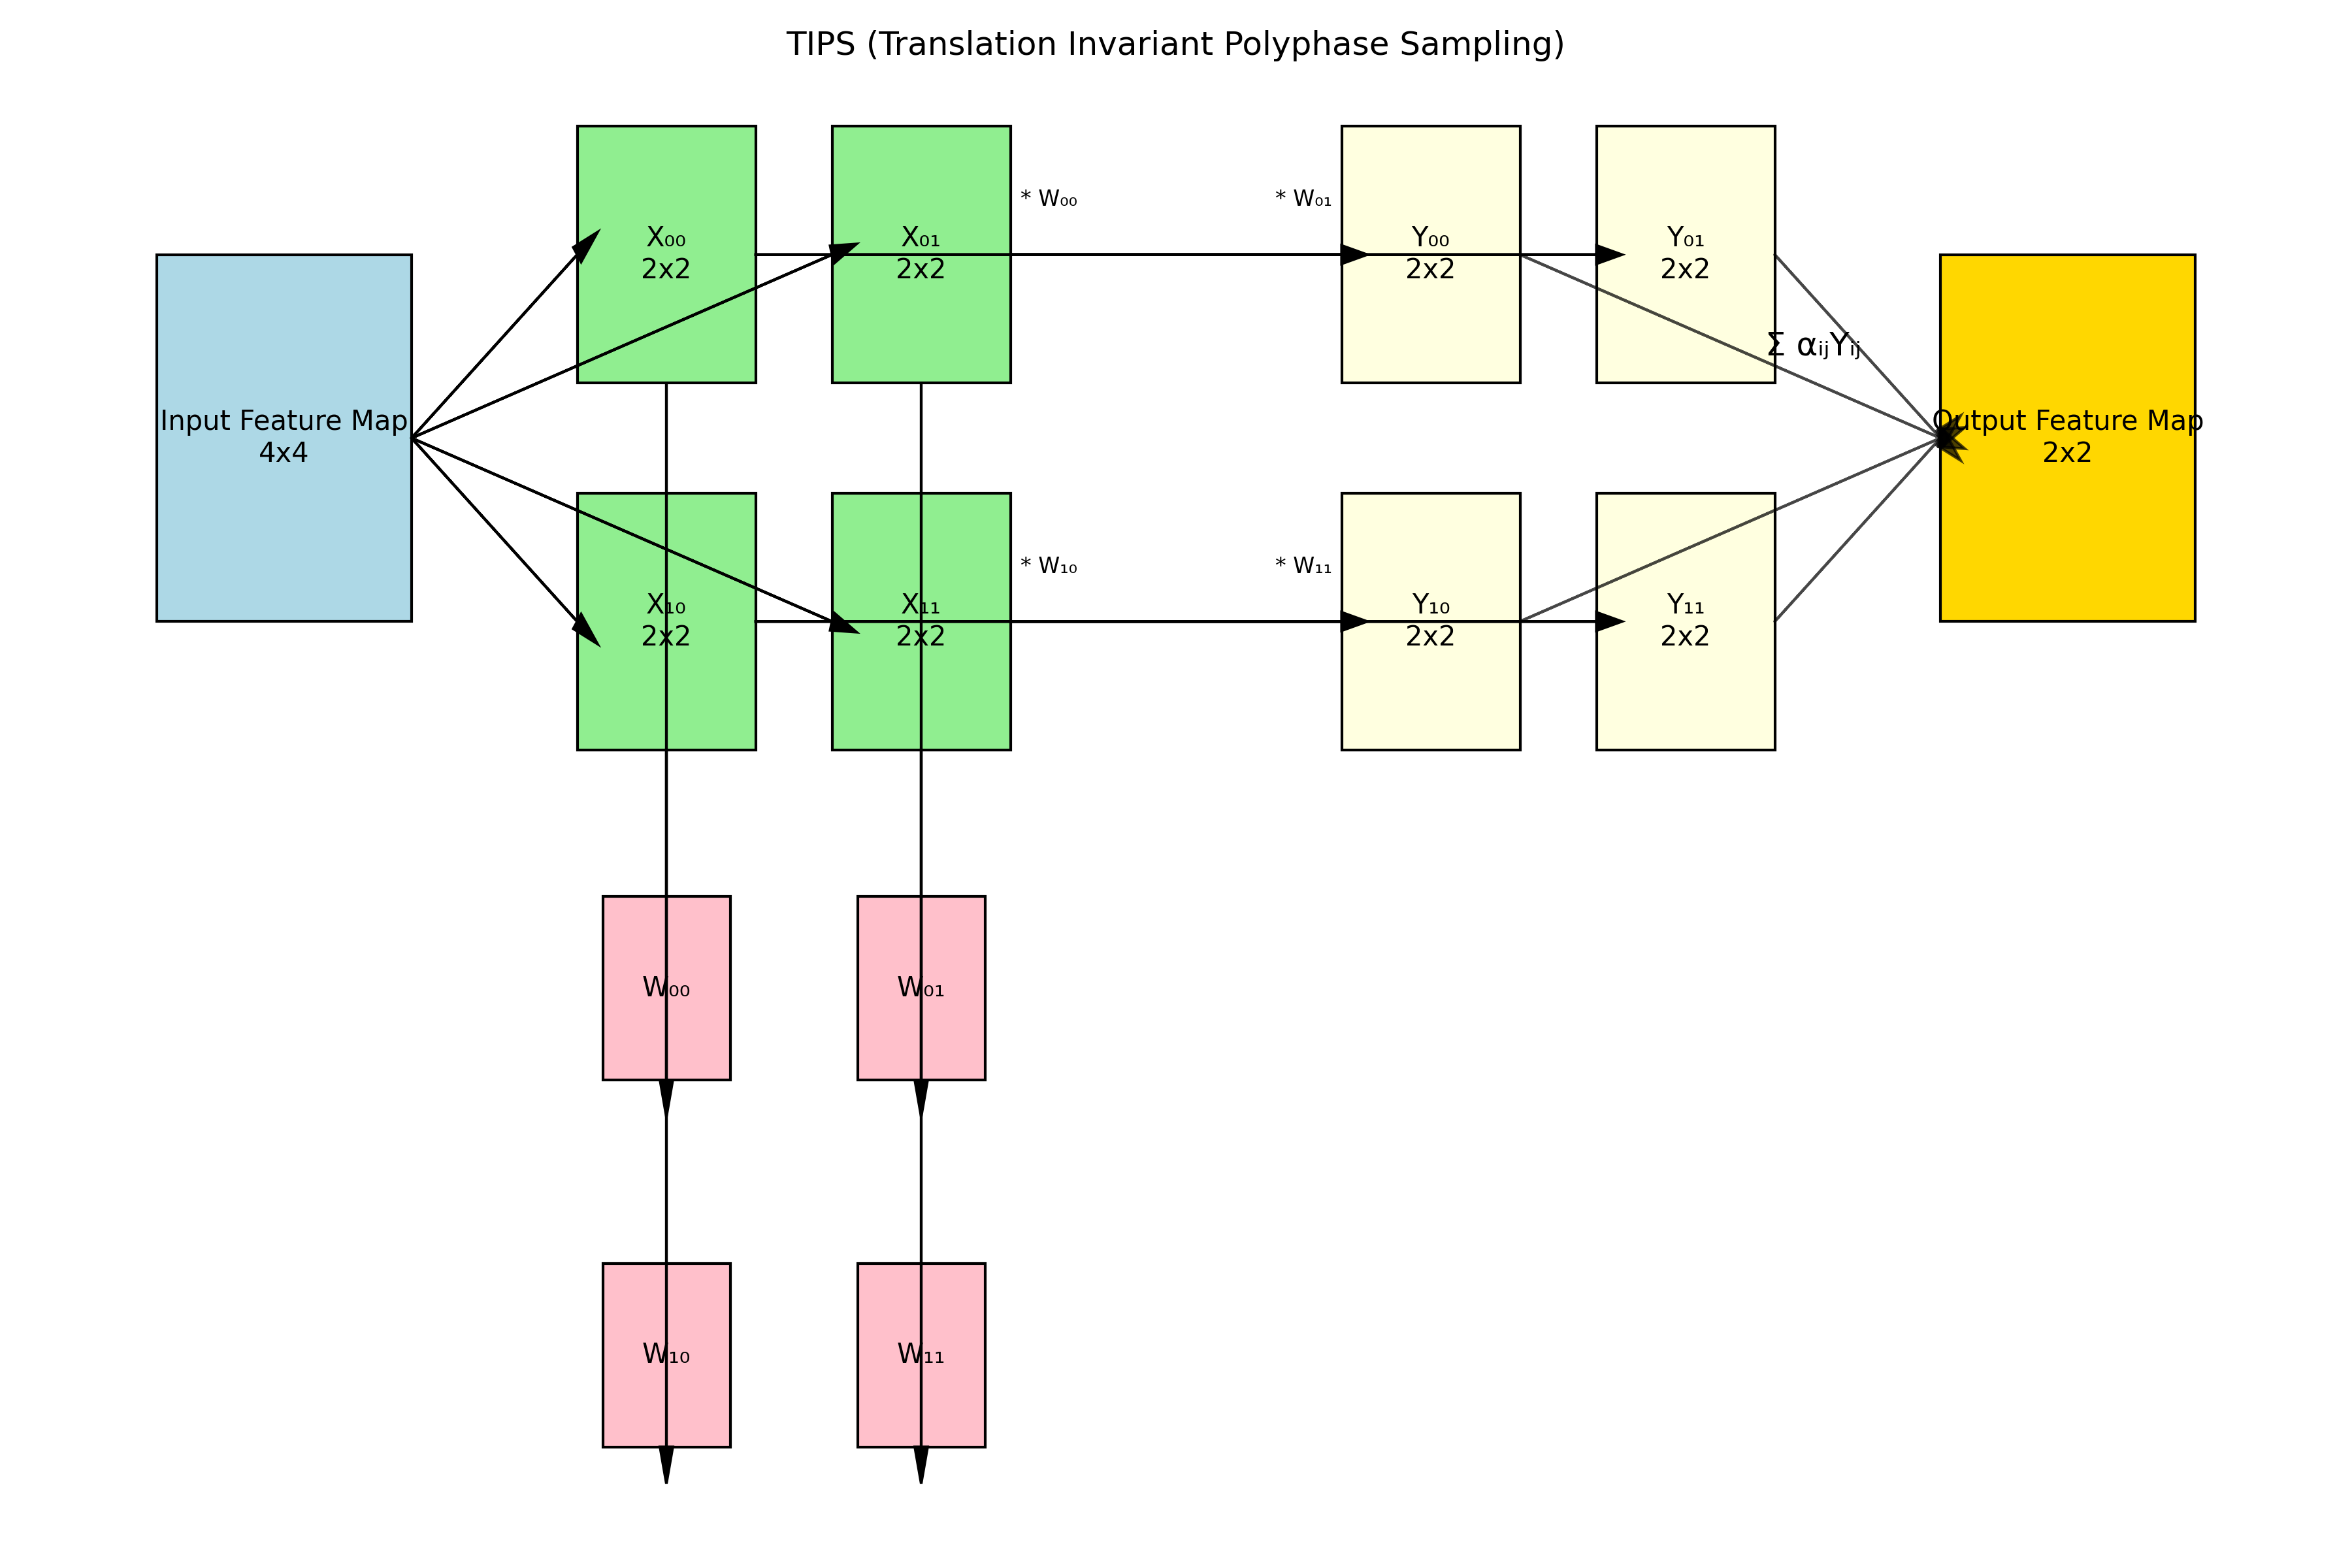
\includegraphics[width=0.9\textwidth]{Dissertation/images/tips_illustration.png}
\caption{Принцип работы TIPS: входная карта признаков разбивается на $s^2$ полифазных компонент (для шага $s$), каждая из которых обрабатывается отдельно, а затем результаты объединяются.}
\label{fig:tips_illustration}
\end{figure}

Основная идея TIPS состоит в следующем:

\begin{enumerate}
    \item Разбиение входной карты признаков на $s^2$ полифазных компонент, соответствующих различным субпиксельным сдвигам (для шага даунсэмплинга $s$).
    \item Независимая обработка каждой полифазной компоненты.
    \item Объединение результатов с использованием весов, которые зависят от конкретного субпиксельного сдвига входного сигнала.
\end{enumerate}

Математически, для входной карты признаков $X[n,m]$ полифазное разложение для шага $s$ дает $s^2$ компонент:

\begin{equation}
X_{p,q}[n,m] = X[sn+p, sm+q]
\end{equation}

где $p, q \in \{0, 1, ..., s-1\}$.

Каждая полифазная компонента $X_{p,q}$ соответствует даунсэмплингу оригинального сигнала с определенным субпиксельным сдвигом. TIPS обрабатывает каждую компоненту отдельным сверточным фильтром:

\begin{equation}
Y_{p,q} = X_{p,q} * W_{p,q}
\end{equation}

где $W_{p,q}$ — обучаемые веса для конкретной полифазной компоненты.

Финальный выход формируется как взвешенная сумма:

\begin{equation}
Y = \sum_{p=0}^{s-1} \sum_{q=0}^{s-1} \alpha_{p,q} \cdot Y_{p,q}
\end{equation}

где $\alpha_{p,q}$ — коэффициенты, зависящие от субпиксельного сдвига входного сигнала. Эти коэффициенты могут быть фиксированными (например, равными $1/s^2$ для равномерного усреднения) или обучаемыми.

Преимущества TIPS по сравнению с BlurPool:

\begin{itemize}
    \item \textbf{Теоретически оптимальный подход}: TIPS основан на теории полифазного представления сигналов и обеспечивает оптимальную реконструкцию для любого субпиксельного сдвига.
    
    \item \textbf{Адаптивность}: TIPS может адаптироваться к специфическим характеристикам данных через обучение весов полифазных фильтров.
    
    \item \textbf{Максимальное сохранение информации}: Благодаря раздельной обработке полифазных компонент, TIPS сохраняет больше информации о высоких частотах по сравнению с BlurPool.
\end{itemize}

Недостатки TIPS:

\begin{itemize}
    \item \textbf{Вычислительная сложность}: TIPS требует в $s^2$ раз больше параметров и вычислений для слоя даунсэмплинга с шагом $s$.
    
    \item \textbf{Сложность реализации}: Интеграция TIPS в существующие архитектуры требует более значительных изменений в коде по сравнению с BlurPool.
\end{itemize}

\subsection{Сравнение методов анти-алиасинга}
\label{theory:anti_aliasing:comparison}

Сравним основные методы анти-алиасинга, используемые в CNN:

\begin{table}[ht]
\centering
\caption{Сравнение методов анти-алиасинга}
\label{tab:antialiasing_comparison}
\begin{tabular}{|l|p{3.5cm}|p{3.5cm}|p{3.5cm}|}
\hline
\textbf{Характеристика} & \textbf{Стандартный даунсэмплинг} & \textbf{BlurPool} & \textbf{TIPS} \\ \hline
Принцип работы & Прямое уменьшение разрешения без фильтрации & Низкочастотная фильтрация перед даунсэмплингом & Полифазное разложение и адаптивная обработка компонент \\ \hline
Теоретическая обоснованность & Низкая & Средняя (на основе классической теории обработки сигналов) & Высокая (на основе полифазного представления) \\ \hline
Вычислительная сложность & Низкая & Низкая-средняя & Высокая \\ \hline
Количество дополнительных параметров & 0 & Минимальное (фиксированные фильтры) & Высокое ($O(s^2)$ на слой) \\ \hline
Влияние на точность классификации & Базовая & Незначительное улучшение или сохранение & Умеренное улучшение \\ \hline
Улучшение инвариантности к сдвигу & - & Значительное & Максимальное \\ \hline
Простота интеграции & - & Высокая & Средняя \\ \hline
\end{tabular}
\end{table}

Обе технологии, BlurPool и TIPS, значительно улучшают инвариантность CNN к пространственным сдвигам, но имеют разный баланс между эффективностью, сложностью и теоретической обоснованностью. BlurPool предлагает простое и вычислительно эффективное решение, которое можно легко интегрировать в существующие архитектуры. TIPS обеспечивает теоретически оптимальную инвариантность к сдвигу, но требует больше вычислительных ресурсов и более сложен в реализации.

В экспериментальной части работы мы проведем сравнительный анализ этих методов на различных архитектурах CNN и задачах, чтобы определить их практическую эффективность в реальных условиях.

